\documentclass[11pt]{article}
\usepackage{ragged2e}
\usepackage[utf8]{inputenc}
\usepackage[catalan]{babel}
\usepackage{graphicx}
\usepackage{array}
\usepackage{afterpage}
\usepackage{listings}
\usepackage{standalone}
\usepackage{caption}
\graphicspath{ {Images/} }

\usepackage[a4paper, total={6in, 8in}]{geometry}

\begin{document}
\begin{titlepage}

\newcommand{\HRule}{\rule{\linewidth}{0.5mm}} % Defines a new command for the horizontal lines, change thickness here

\center % Center everything on the page
 
%----------------------------------------------------------------------------------------
%	HEADING SECTIONS
%----------------------------------------------------------------------------------------

\textsc{\LARGE Universitat de Lleida}\\[1cm] % Name of your university/college

\includegraphics[scale=0.75]{Images/eps.png}\\[0.65cm] % Include a department/university logo - this will require the graphicx package
\textsc{\Large Grau en Enginyeria Informàtica}\\[0.3cm] % Major heading such as course name
\textsc{\large Intel·ligència Artificial}\\[0.5cm] % Minor heading such as course title

%----------------------------------------------------------------------------------------
%	TITLE SECTION
%----------------------------------------------------------------------------------------

\HRule \\[0.4cm]
{\huge \bfseries Tercera pràctica d'Intel·ligència Artificial}\\[0.0cm]
% Title of your document
\HRule \\[1cm] 

%----------------------------------------------------------------------------------------
\begin{minipage}{0.4\textwidth}
\begin{flushleft} \large
\emph{Autors:}\\
Jaume Giralt Barbé\\
Jordi Onrubia Palacios\\
\end{flushleft}
\end{minipage}
~
\begin{minipage}{0.4\textwidth}
\begin{flushright} \large
\emph{Professor:} \\
Carlos Jose Ansotegui Gil\\
Josep Pon Farreny
% Supervisor's Name
\end{flushright}
\end{minipage}\\[4cm]

%----------------------------------------------------------------------------------------
%	DATE SECTION
%----------------------------------------------------------------------------------------
{\large \today}\\[3cm] % Date, change the \today to a set date if you want to be precise
\vfill % Fill the rest of the page with whitespace
\end{titlepage}
\newpage
\tableofcontents
\listoftables
\listoffigures
\clearpage
\newpage
\justify
\section{Contingut}
	\subsection{Contingut Principal}
		El contingut principal es centre en els següents fitxers:
		\begin{itemize}
			\item \textbf{Tree Predict:} Aquest és el fitxer principal de la pràctica, el que ens ha donat mes feina per fer la realització. Són mètodes transparents de classificar observacions que després d'entrenar-lo amb dades amb característiques similars ho ordena fent servir sentències \textit{if then} formant un \textbf{arbre}.
			\item \textbf{Bayesian Learning:} Aquest fitxer està implementat un altre mètode de aprenentatge supervisat. Amb aquest mètode podem classificar si una paraula/frase pertany a una categoria o a una altra després d'entrenar-lo. Un exemple del seu funcionament a la vida real serie el Anti-SPAM del correu electrònic.
			\item \textbf{K-Means Cluster:} L'algorisme K-means és un mètode d'agrupament que té com a objectiu la partició d'un conjunt n observacions en k grups en el qual cada observació pertany al grup més proper a la mitjana. És un mètode d'aprenentatge no supervisat.
		\end{itemize}
	\subsection{Contingut Secundari}
		A més a més de els fitxers esmentats anteriorment, també hem afegit un joc de proves per realitzar l'avaluació experimental. També hem afegit scripts utilitzats per extreure les dades i per crear els gràfics amb l'eina GNU-Plot.
\newpage
\section{Decisions de disseny}
	\subsection{Tree Predict}
		En aquest document és on hem hagut d'implementar més funcions per la pràctica. En primer lloc, hem implementat les funcions \textbf{buildTree} i \textbf{buildTreeIterative}, que són les funcions encarregades de muntar el arbre a partir de les dades d'entrada. La funció buildtree rep d'entrada un conjunt de dades i les divideix en columnes segons la impuresa ja que a més decrement, millor són els subconjunts. Aquesta impuresa ve donada al utilitzar la funció amb les funcions de l'index de Gini o l'Entropia. El resultat d'aquesta funció és un arbre amb les seves branques verdader i fals on es mostra el resultat de les preguntes realitzades. En la versió iterativa del algoritme hem aplicat els coneixements adquirits en l'assignatura de Algorítmica i Complexitat on ens explicaven que un dels mètodes per passar una funció recursiva a iterativa era la utilització de piles per simular les crides recursives. Es per això que hem implementat la nostra pròpia pila per fer aquesta funció. Una altra funció que hem hagut d'implementar és la funció \textbf{classifier} que consisteix en donat unes característiques i un arbre, ens dóna l'atribut que volem cercar. Aquesta funció la farem servir amb la funció de \textbf{testPerformance} que donat dos sets de característiques, entrenem un arbre amb el \textit{trainingSet} i per cada conjunt de característiques del \textit{testSet} cridem a l'anterior funció esmentada i comprovem si ens dóna l'argument correcte. Amb aquesta funció i amb funcions auxiliars és com hem pogut realitzar l'avaluació experimental.
		
	\subsection{Bayesian Learning}
		
	\subsection{K-Means Cluster}

\section{Avaluació Experimental}
	\begin{table}[!h]
\begin{minipage}[b]{0.4\linewidth}
\centering
\resizebox{9cm}{!}{
\begin{tabular}{|c|c|}\hline
Percentatge TrainSet & Percentatge Good 	\\\hline
0.1	 & 	19.04	 \\\hline
0.2	 & 	37.5	 \\\hline
0.3	 & 	44.89	 \\\hline
0.4	 & 	35.71	 \\\hline
0.5	 & 	40.0	 \\\hline
0.6	 & 	53.57	 \\\hline
0.7	 & 	47.61	 \\\hline
0.8	 & 	57.14	 \\\hline
0.9	 & 	57.14	 \\\hline
\end{tabular}
}
\caption{Taula per al test de les variables de tipus categoria}
\label{tab:astartable}
\end{minipage}\hfill
\begin{minipage}[b]{0.4\linewidth}
\centering
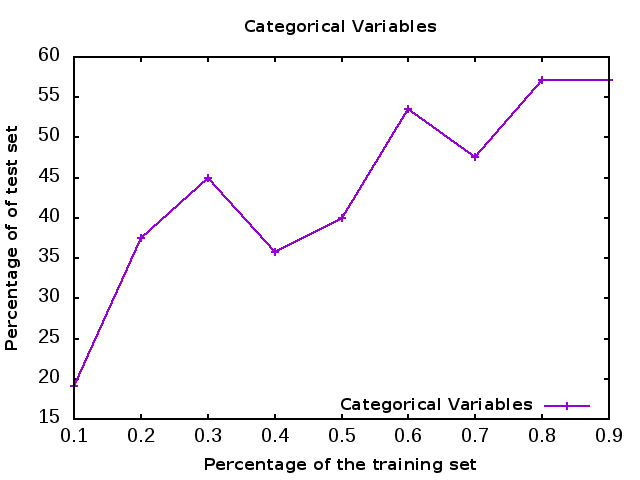
\includegraphics[width=1.2\linewidth]{Images/bridge.png}
\captionof{figure}{Gràfica per al test de les variables de tipus categoria}
\label{fig:astar}
 \end{minipage}
\end{table}
\end{document}